\documentclass[11pt,a4paper]{article}
\usepackage[utf8]{inputenc}
\usepackage{amsmath, amssymb, amsthm, graphicx, float}
\graphicspath{ {../../} }
\usepackage{bm}
\usepackage[margin=2.5cm]{geometry} 
\usepackage{microtype}        
\usepackage{hyperref}        
\usepackage[capitalize,noabbrev]{cleveref} 
\usepackage{booktabs}      


\hypersetup{
    colorlinks=true,
    linkcolor=black,
    citecolor=black,
    urlcolor=blue
}

\title{Robust Portfolio Optimization: From Mean-Variance to Hierarchical Risk Parity}
\author{Sacha Reymond}
\date{}

\begin{document}

\maketitle

\section{Mean-Variance Optimization}
\subsection{Return Estimation and Covariance Structure}
Let $P_t^{(i)}$ denote the adjusted close price of asset $i$ at time $t$. We compute discrete returns as:
\begin{equation}
r_t^{(i)} = \frac{P_t^{(i)} - P_{t-1}^{(i)}}{P_{t-1}^{(i)}}, \quad \text{or} \quad r_t^{(i)} = \log\left(\frac{P_t^{(i)}}{P_{t-1}^{(i)}}\right) \quad \text{(log returns)}.
\end{equation}
The sample covariance matrix $S$ is the unbiased estimator:
\begin{equation}
S = \frac{1}{T-1} \sum_{t=1}^T (r_t - \bar{r})(r_t - \bar{r})^T, \quad \bar{r} = \frac{1}{T} \sum_{t=1}^T r_t.
\end{equation}
In the high-dimensional regime where $N \approx T$, $S$ is ill-conditioned, motivating the Ledoit-Wolf shrinkage (Section~1.3).
\subsection{The Primal Optimization Problem}
Consider a universe of $N$ liquid assets. Let $\mathbf{w} \in \mathbb{R}^N$ denote the portfolio weight vector, $\bm{\mu} \in \mathbb{R}^N$ the vector of expected returns, and $\Sigma \in \mathbb{S}_{++}^N$ the covariance matrix (assumed positive definite). The long-only mean-variance problem is:

\begin{equation}
\begin{aligned}
& \min_{\mathbf{w}} \quad \frac{1}{2} \mathbf{w}^T \Sigma \mathbf{w} \\
& \text{s.t.} \quad \mathbf{w}^T \mathbf{1} = 1 \\
& \quad \quad \mathbf{w}^T \bm{\mu} = r_{target} \\
& \quad \quad w_i \geq 0, \quad \forall i \in \{1, \dots, N\}
\end{aligned}
\end{equation}

\subsection{The Lagrangian and KKT Conditions}
We first derive the solution for the unconstrained case (without non-negativity constraints). The Lagrangian is:
\begin{equation}
\mathcal{L}_0(\mathbf{w}, \lambda, \gamma) = \frac{1}{2} \mathbf{w}^T \Sigma \mathbf{w} - \lambda(\mathbf{w}^T \mathbf{1} - 1) - \gamma(\mathbf{w}^T \bm{\mu} - r_{target})
\end{equation}

Taking the gradient with respect to $\mathbf{w}$ and setting it to zero (stationarity condition), we obtain:
\begin{equation}
\nabla_{\mathbf{w}} \mathcal{L}_0 = \Sigma \mathbf{w} - \lambda \mathbf{1} - \gamma \bm{\mu} = 0
\end{equation}
which implies:
\begin{equation}
\mathbf{w} = \Sigma^{-1}(\lambda \mathbf{1} + \gamma \bm{\mu}) \label{eq:weight_unconstrained}
\end{equation}

Substituting into the primal feasibility constraints $\mathbf{w}^T \mathbf{1} = 1$ and $\mathbf{w}^T \bm{\mu} = r_{target}$, we obtain:
\begin{align}
\mathbf{1}^T \Sigma^{-1} (\lambda \mathbf{1} + \gamma \bm{\mu}) &= 1 \label{eq:constraint1} \\
\bm{\mu}^T \Sigma^{-1} (\lambda \mathbf{1} + \gamma \bm{\mu}) &= r_{target} \label{eq:constraint2}
\end{align}

Defining the following scalar quantities:
\begin{align}
A &= \mathbf{1}^T \Sigma^{-1} \mathbf{1} \\
B &= \mathbf{1}^T \Sigma^{-1} \bm{\mu} = \bm{\mu}^T \Sigma^{-1} \mathbf{1} \\
C &= \bm{\mu}^T \Sigma^{-1} \bm{\mu}
\end{align}

Equations~\eqref{eq:constraint1} and~\eqref{eq:constraint2} can be rewritten as the linear system:
\begin{equation}
\begin{bmatrix}
A & B \\
B & C
\end{bmatrix}
\begin{bmatrix}
\lambda \\
\gamma
\end{bmatrix}
=
\begin{bmatrix}
1 \\
r_{target}
\end{bmatrix}
\end{equation}

We solve this system using Cramer's rule. The determinant is:
\begin{equation}
\Delta = \begin{vmatrix}
A & B \\
B & C
\end{vmatrix} = AC - B^2
\end{equation}

The solutions are:
\begin{align}
\lambda &= \frac{1}{\Delta} \begin{vmatrix}
1 & B \\
r_{target} & C
\end{vmatrix} = \frac{C - r_{target}B}{AC - B^2} \label{eq:lambda} \\
\gamma &= \frac{1}{\Delta} \begin{vmatrix}
A & 1 \\
B & r_{target}
\end{vmatrix} = \frac{Ar_{target} - B}{AC - B^2} \label{eq:gamma}
\end{align}


Substituting equations~\eqref{eq:lambda} and~\eqref{eq:gamma} into equation~\eqref{eq:weight_unconstrained}, we obtain the optimal weight vector:
\begin{equation}
\mathbf{w} = \Sigma^{-1}\left(\frac{C - r_{target}B}{AC - B^2} \mathbf{1} + \frac{Ar_{target} - B}{AC - B^2} \bm{\mu}\right)
\end{equation}

However, we need to add the non-negativity constraints. Indeed, the weight vector $\mathbf{w}$ is not guaranteed to be non-negative, and we require a long-only portfolio (i.e., $w_i \geq 0$ for all $i$). To solve this Quadratic Programming (QP) problem, we define the Lagrangian $\mathcal{L}$ with multipliers $\lambda$ (budget), $\gamma$ (return), and $\mathbf{z}$ (non-negativity):


\begin{equation}
\mathcal{L}(\mathbf{w}, \lambda, \gamma, \mathbf{z}) = \frac{1}{2} \mathbf{w}^T \Sigma \mathbf{w} - \lambda(\mathbf{w}^T \mathbf{1} - 1) - \gamma(\mathbf{w}^T \bm{\mu} - r_{target}) - \mathbf{z}^T \mathbf{w}
\end{equation}


The Karush-Kuhn-Tucker (KKT) first-order necessary conditions for optimality are:
\begin{enumerate}
    \item \textbf{Stationarity:} $\nabla_{\mathbf{w}} \mathcal{L} = \Sigma \mathbf{w} - \lambda \mathbf{1} - \gamma \bm{\mu} - \mathbf{z} = 0$
    \item \textbf{Primal Feasibility:} $\mathbf{w}^T \mathbf{1} = 1$ and $\mathbf{w}^T \bm{\mu} = r_{target}$
    \item \textbf{Dual Feasibility:} $z_i \geq 0$
    \item \textbf{Complementary Slackness:} $z_i w_i = 0, \quad \forall i$
\end{enumerate}



\subsection{Spectral Instability and Ledoit-Wolf Shrinkage}
The sample covariance $S$ is ill-conditioned in high dimensions. Under its spectral decomposition $S = V \Lambda V^T$, the optimal weights $\mathbf{w}^* \propto \Sigma^{-1}(\lambda \mathbf{1} + \gamma \bm{\mu})$ exhibit catastrophic sensitivity to small eigenvalues: if $\lambda_{\min} \to 0$, then $\|\mathbf{w}^*\| \to \infty$ (the "corner solution" problem).

The Ledoit-Wolf shrinkage estimator regularizes the spectrum by shrinking $S$ toward a structured target $F = \bar{\sigma}^2 I$:
\begin{equation}
\hat{\Sigma}_{\text{LW}} = (1 - \delta) S + \delta F,
\end{equation}
which bounds the condition number $\kappa(\hat{\Sigma}_{\text{LW}}) \leq \kappa_{\max}$ and stabilizes the KKT system. 

\subsection{Derivation of the Optimal Shrinkage Intensity}

\subsubsection{Loss Function and First-Order Condition}
The loss function $L(\delta)$ is defined as:
\begin{equation}
L(\delta) = \mathbb{E}[\|\hat{\Sigma}(\delta) - \Sigma\|^2_{\text{Fro}}] = \mathbb{E}[\operatorname{Tr}((\hat{\Sigma}(\delta) - \Sigma)^T (\hat{\Sigma}(\delta) - \Sigma))]
\end{equation}

Defining the error terms $A = S - \Sigma$ and $B = F - S$, the estimator error can be rewritten as:
\begin{equation}
\hat{\Sigma}(\delta) - \Sigma = (S - \Sigma) + \delta(F - S) = A + \delta B
\end{equation}

Expanding the trace via linearity:
\begin{equation}
L(\delta) = \mathbb{E}[\operatorname{Tr}(A^T A)] + 2\delta \mathbb{E}[\operatorname{Tr}(B^T A)] + \delta^2 \mathbb{E}[\operatorname{Tr}(B^T B)]
\end{equation}

The first-order condition $\frac{dL}{d\delta} = 0$ yields the theoretical optimal intensity:
\begin{equation}
\delta^* = -\frac{\mathbb{E}[\operatorname{Tr}(B^T A)]}{\mathbb{E}[\operatorname{Tr}(B^T B)]}
\end{equation}

\subsubsection{Decomposition into \texorpdfstring{$\pi$, $\rho$, and $\gamma$}{π, ρ, and γ} Parameters}
To make this solution computable, we decompose the numerator and denominator into three fundamental parameters.

\paragraph{The parameter $\gamma$ (Distance to structure):}
This represents the expected energy of the displacement toward the target:
\begin{equation}
\gamma = \mathbb{E}[\|F - S\|^2_{\text{Fro}}] = \mathbb{E}[\operatorname{Tr}(B^T B)]
\end{equation}

\paragraph{The parameter $\pi$ (Sample noise):}
This corresponds to the sum of the variances of the elements in the sample matrix:
\begin{equation}
\pi = \sum_{i,j} \operatorname{Var}(s_{ij}) = \mathbb{E}[\operatorname{Tr}(S^T S)] - \operatorname{Tr}(\Sigma^T \Sigma)
\end{equation}

\paragraph{The parameter $\rho$ (Stochasticity correction):}
Since $F$ is constructed from $S$, it shares a portion of the sampling error. This term captures the covariance between the errors of the target and the sample:
\begin{equation}
\rho = \sum_{i,j} \operatorname{cov}(f_{ij}, s_{ij}) = \mathbb{E}[\operatorname{Tr}(F^T S)] - \operatorname{Tr}(F^T \Sigma)
\end{equation}

\subsubsection{Final Synthesis}
Substituting these definitions into the expression for $\delta^*$, we find:
\begin{equation}
\mathbb{E}[\operatorname{Tr}(B^T A)] = \mathbb{E}[\operatorname{Tr}((F-S)^T(S-\Sigma))] = \rho - \pi
\end{equation}
Which leads to the optimal Ledoit-Wolf intensity:
\begin{equation}
    \hat{\delta}^* = \max \left\{ 0, \min \left\{ 1, \frac{1}{T} \cdot \frac{\hat{\pi} - \hat{\rho}}{\hat{\gamma}} \right\} \right\},
\end{equation}
where $\hat{\pi}$, $\hat{\rho}$, and $\hat{\gamma}$ are consistent estimators. This formulation ensures:
\begin{equation}
\lim_{T \to \infty} \hat{\delta}^* = 0,
\end{equation}

\subsubsection{Implementation Interpretation}
The intensity $\delta^*$ is the ratio of the net estimation error $(\pi - \rho)$ to the distance from the target structure $\gamma$. In our empirical application to French equities, if the market is highly volatile (high $\pi$) or the time series is short, the shrinkage becomes more aggressive ($\delta \to 1$). 

The inclusion of $\rho$ is vital: it ensures that if the target $F$ drifts in the same direction as the error in $S$, the shrinkage intensity is reduced to avoid reinforcing a pre-existing statistical bias.

\subsubsection{The Finite-Sample Estimator}
In the population limit, the parameters $\pi$, $\rho$, and $\gamma$ represent asymptotic quantities. However, for a practical implementation with a sample of size $T$, we must acknowledge that the estimation variance of the sample covariance entries $s_{ij}$ is $O(1/T)$. 

To maintain consistency with the Ledoit-Wolf~(2004) framework, we define the practical shrinkage intensity as:
\begin{equation}
\hat{\delta}^* = \max \left( 0, \min \left( 1, \frac{1}{T} \frac{\hat{\pi} - \hat{\rho}}{\hat{\gamma}} \right) \right)
\end{equation}
where $\hat{\pi}$, $\hat{\rho}$, and $\hat{\gamma}$ are consistent estimators of their respective population parameters. 

This formulation yields a critical asymptotic result:
\begin{equation}
\lim_{T \to \infty} \hat{\delta}^* = 0
\end{equation}
This implies that as the number of observations $T$ grows, the sample covariance $S$ converges in probability to the true covariance $\Sigma$, and the necessity for regularization through the target $F$ vanishes. This ensures that our optimizer remains statistically consistent while providing maximum stability in the high-dimensional regime where $N \approx T$.

\newpage
\section{Efficient Frontier}
\subsection{The Efficient Frontier}
For a universe of $N = 50$ assets, we compute the efficient frontier by solving the mean-variance problem~\eqref{eq:weight_unconstrained} over a grid of target returns $r_{\text{target}} \in [r_{\min}, r_{\max}]$. Each point $({\sigma_p}, \mathbb{E}[R_p])$ on the frontier represents the minimum-variance portfolio achieving expected return $\mathbb{E}[R_p]$.

Figure~\ref{fig:results} visualizes this tradeoff. Points \emph{above} the frontier are unattainable; points \emph{below} are inefficient (i.e., dominated by a portfolio with higher return at the same risk). Individual assets (plotted as markers) lie strictly below the frontier, confirming the gains from diversification.

\begin{figure}[H]
    \centering
    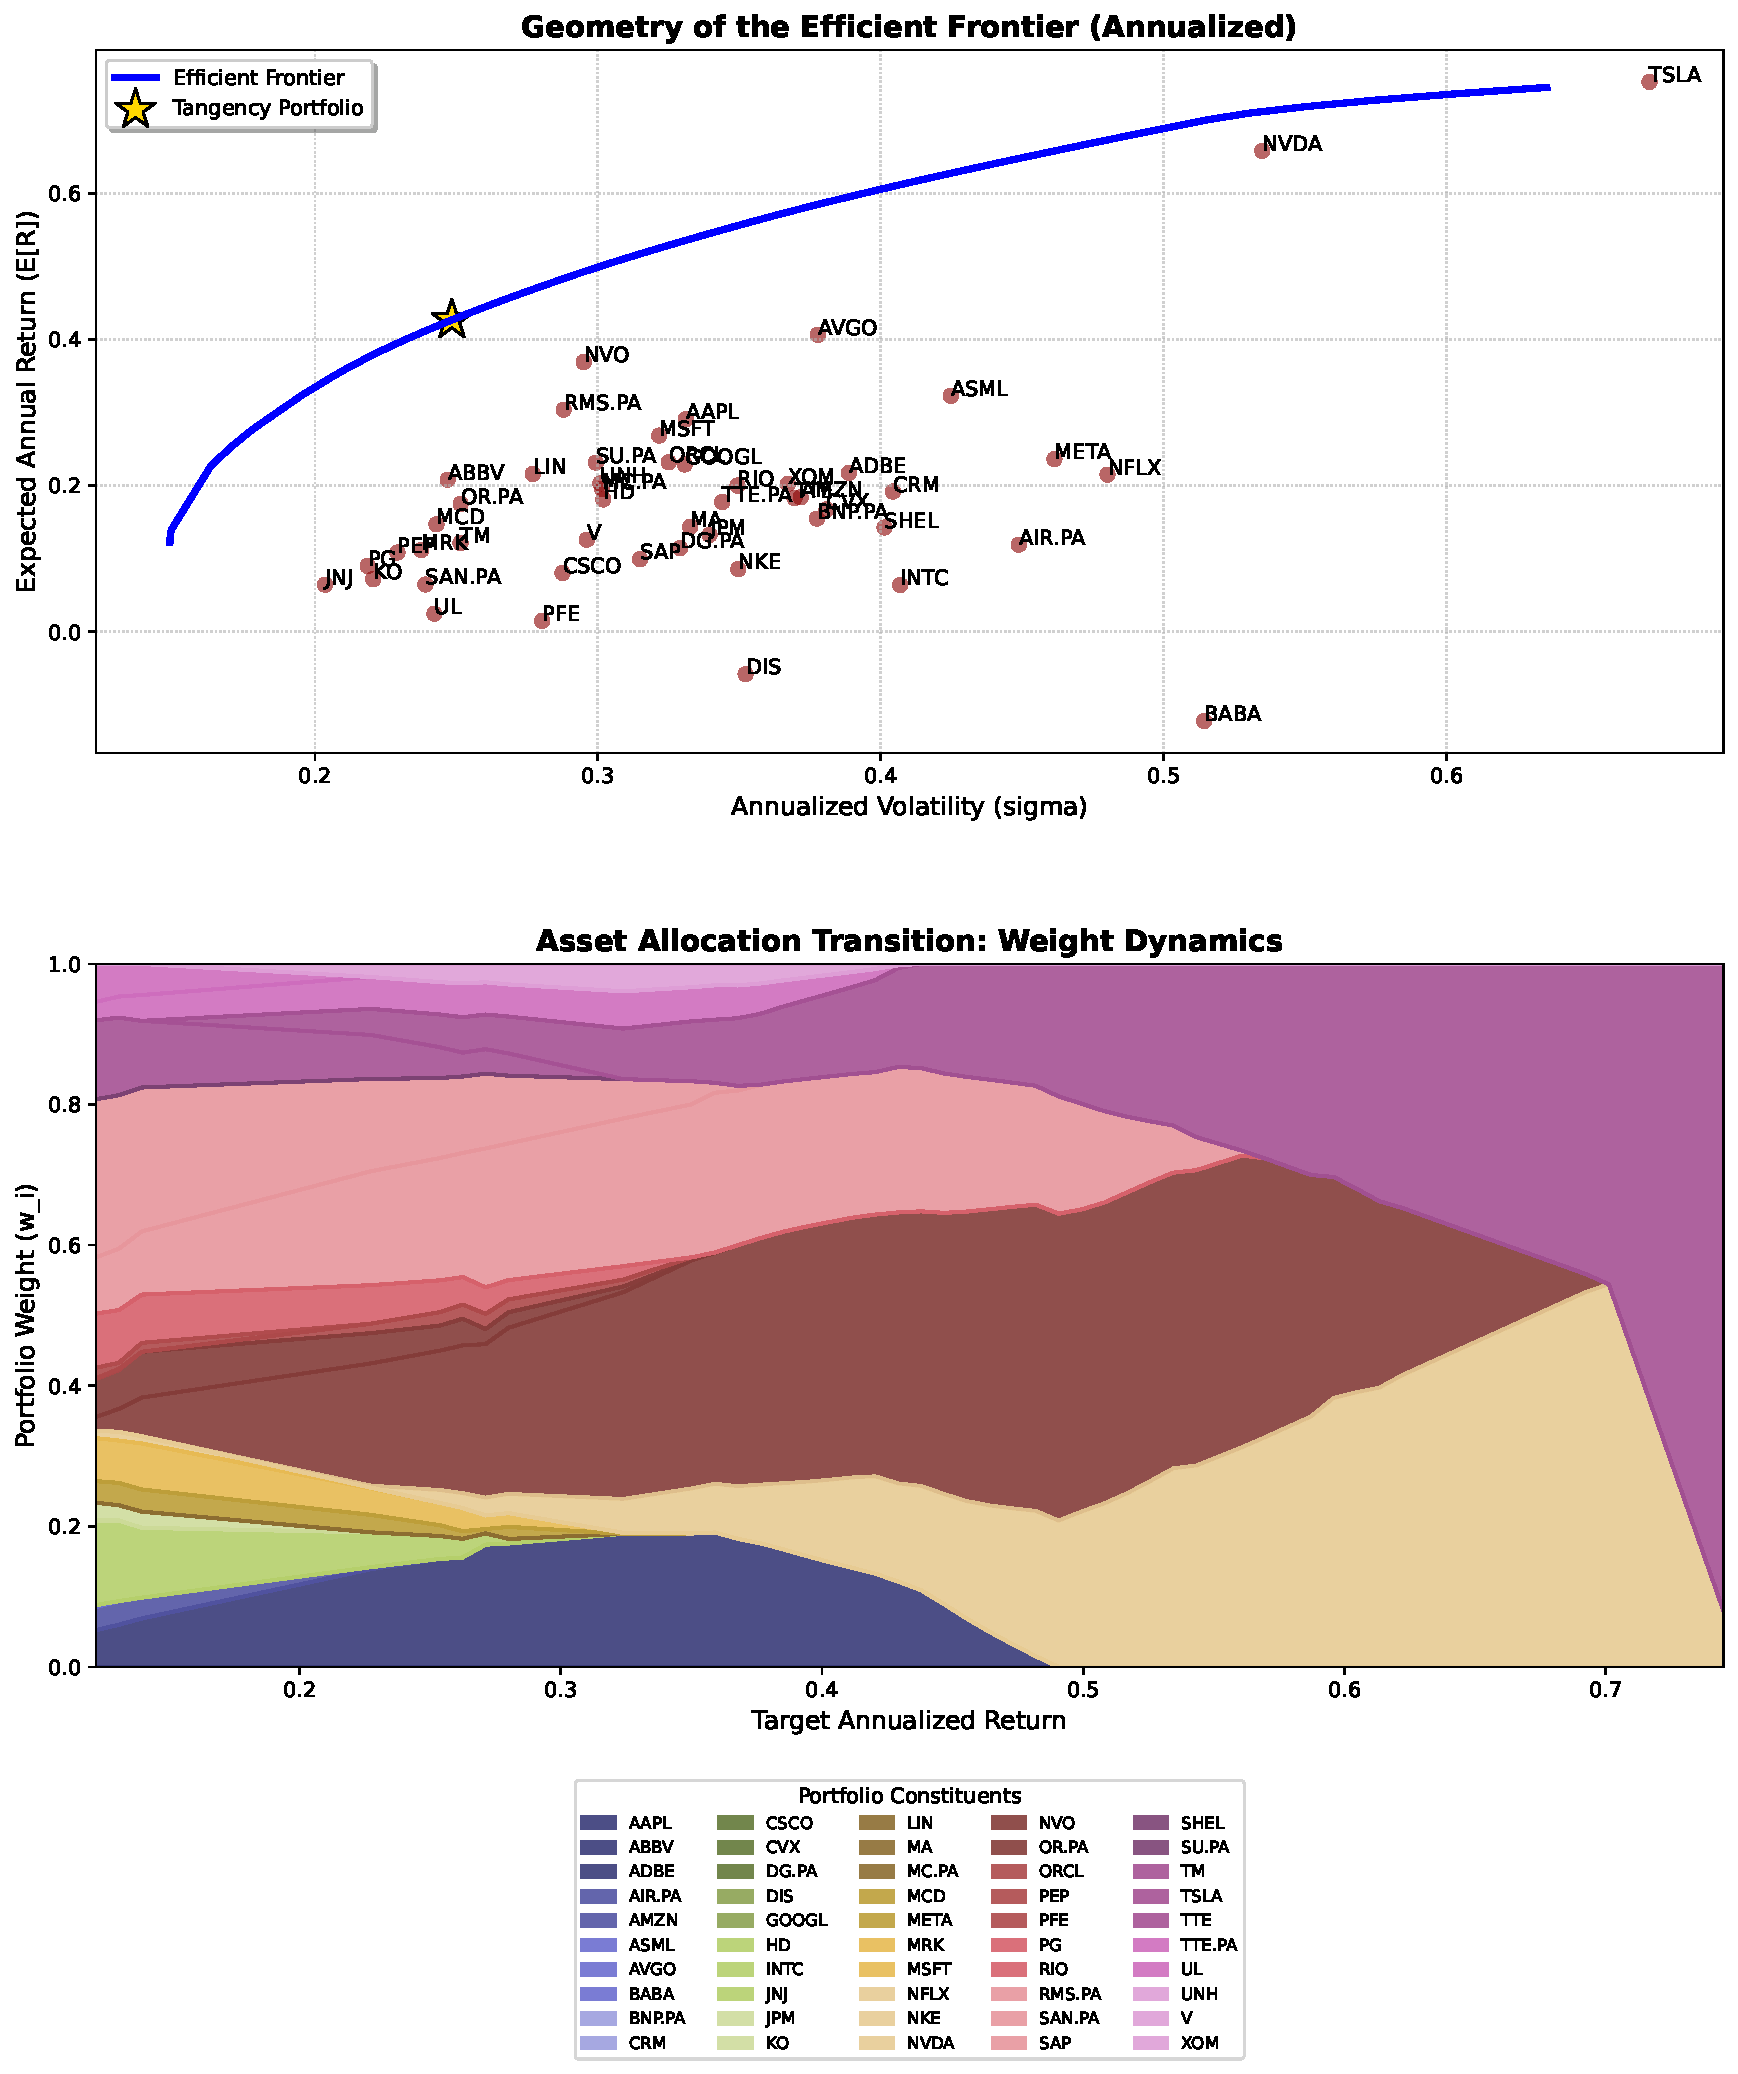
\includegraphics[width=0.8\textwidth]{../../efficient_frontier.pdf}
    \caption{Efficient Frontier visualization.}
    \label{fig:results}
\end{figure}
\subsection{The Tangency Portfolio}
The tangency portfolio is represented by the star on the efficient frontier.
It's the portfolio that maximizes the Sharpe ratio. According to Tobin Separation Theorem, the best way to allocate money 
is to find the portfolio with the best sharpe ratio regardless of risk aversion and then
allocate money in either that portfolio or risk-free assets depending on the investor's risk aversion.
It states that for any level of risk, you are to get a higher expected return by mixing the tangency portfolio with risk free assets than 
by picking a suboptimal point on the Markowitz frontier.

The Sharpe ratio is defined as:
\begin{equation}
SR = \frac{R_p - R_f}{\sigma_p} = \frac{\mathbf{w}^T \bm{\mu} - R_f}{\sqrt{\mathbf{w}^T \Sigma \mathbf{w}}}
\end{equation}
where $R_p$ is the expected return of the portfolio, $R_f$ is the risk-free rate and $\sigma_p$ is the standard deviation of the portfolio.
Directly maximizing $SR(\mathbf{w})$ via SLSQP is numerically unstable due to the square root in the denominator. We transform the problem: define $k$ such that $k(\mathbf{w}^T \bm{\mu} - R_f) = 1$, and substitute $\mathbf{y} = k\mathbf{w}$. Then:
\begin{equation}
SR = \frac{1}{\sqrt{\mathbf{y}^T \Sigma \mathbf{y}}},
\end{equation}
so maximizing $SR$ is equivalent to minimizing $\mathbf{y}^T \Sigma \mathbf{y}$ subject to $\mathbf{y}^T \mathbf{1} = k$ and $(\bm{\mu} - R_f)^T \mathbf{y} = 1$. This is a standard QP.

\section{Risk Decomposition}
We will now chiefly consider the case of the tangency portfolio.
Each asset comes with a certain level of risk.
We will consider three key metrics to quantify the risk of an asset:
\begin{itemize}
    \item The Marginal Contribution to Risk (MCR)
    \item The Percentage Contribution to Risk (PCR)
    \item The Component Contribution to Risk (CCR)
\end{itemize}

The MCR is the contribution of an asset to the total risk of the portfolio. It is calculated with the formula:
\begin{equation}
MCR_i = \frac{\partial \sigma_p}{\partial w_i}
\end{equation}

\begin{equation}
\sigma_p = \sqrt{\mathbf{w}^T \Sigma \mathbf{w}}
\end{equation}

\begin{equation}
\frac{\partial \mathbf{w}^T \Sigma \mathbf{w}}{\partial \mathbf{w}} = 2 \Sigma \mathbf{w}
\end{equation}

\begin{equation}
MCR = \frac{\partial \mathbf{w}^T \Sigma \mathbf{w}}{2 \sqrt{\mathbf{w}^T \Sigma \mathbf{w}}} = \frac{2 \Sigma \mathbf{w}}{2 \sqrt{\mathbf{w}^T \Sigma \mathbf{w}}} = \frac{\Sigma \mathbf{w}}{\sigma_p}
\end{equation}

\begin{equation}
MCR_i = \frac{(\Sigma \mathbf{w})_i}{\sigma_p}
\end{equation}

The PCR is the contribution of an asset to the total risk of the portfolio expressed as a percentage.

According to Euler's theorem for homogeneous functions, we have:

\begin{equation}
\sigma_p = \sum_{i=1}^N w_i \frac{\partial \sigma_p}{\partial w_i} = \sum_{i=1}^N w_i MCR_i
\end{equation}
Therefore the PCR is given by:
\begin{equation}
PCR_i = \frac{w_i MCR_i}{\sigma_p}
\end{equation}
and we can note:
\begin{equation}
\sum_{i=1}^N PCR_i = 1
\end{equation}
Also :
\begin{equation}
    PCR_i = \frac{w_i (\Sigma \mathbf{w})_i}{\sigma_p^2}
\end{equation}

And finally the CCR is actual amount of a portfolio's total risk that is attribuable to a specific asset. And thus:
\begin{equation}
    CCR_i = w_i MCR_i = \frac{w_i (\Sigma \mathbf{w})_i}{\sigma_p}
\end{equation}
It is notable that:
\begin{equation}
\sum_{i=1}^N CCR_i = \sigma_p
\end{equation}






\section{Black-Litterman Model}

The Black-Litterman model is a Bayesian approach to portfolio optimization.
It is a two-step process:
\begin{itemize}
    \item First we estimate the expected returns of the assets.
    \item Then we use the expected returns and our personal views to estimate the optimal weights of the portfolio.
\end{itemize}

\subsection{Estimating the Expected Returns}
The first step is to estimate the expected returns of the assets.
We can use the following formula:
\begin{equation}
    \bm{\Pi} = \lambda \Sigma \mathbf{w}_{market}
\end{equation}
\noindent
Where $\lambda$ is the risk aversion coefficient and $\mathbf{w}_{market}$ is the market weights.

To estimate the market weights we extract the number of shares outstanding and multiply it by the latest close price we're interested in.
This gives us the market capitalization of each asset and we then divide it by the sum of the market caps of all the assets we consider.

To estimate the risk aversion coefficient we use the following formula:
\begin{equation}
    \lambda = \frac{[R_p] - R_f}{\sigma_{mkt}^2}
\end{equation}
Otherwise:
\begin{equation}
    \lambda = \frac{SR(r_{mkt})}{\sigma_{mkt}}
\end{equation}
$\lambda$ can be seen as the gradient of the investor's preferences.

Let's show how this formula is derived.

Let's consider the Risk-Adjusted Return (Utility) function. We define U as:
\begin{equation}
    U(w) = \mathbf{w}^T \mathbf{\mu} - \frac{\lambda}{2} \mathbf{w}^T \Sigma \mathbf{w}
\end{equation}
We set up the Lagrangian just like we did in the Mean-Variance Optimization section.
However here we know the weights and are interested in finding the expected returns that maximize the utility function.
We thus get:
\begin{equation}
    \bm{\Pi} = \lambda \Sigma \mathbf{w}_{market} + \gamma \mathbf{1}
\end{equation}

What we are interested in is the excess return relative to the risk-free rate. 
Let's prove that in that case, we have to take $\gamma = 0$:
At the optimum,
\begin{equation}
\mathbf{\mu} - \lambda \Sigma \mathbf{w}_{market} = \gamma \mathbf{1}
\end{equation}
However if we consider that all our assets are risk-free, we have $\Sigma = 0$ since they have no variance.
So $\mathbf{\mu} = \gamma \mathbf{1}$ and in that case $\mathbf{\mu} = R_f \mathbf{1}$.
That leads to $\gamma = R_f$.
Thus if we only consider the excess return over the return offered by risk-free assets we effectively have to set $\gamma = 0$ to avoid an arbitrage opportunity.

We thus get:
\begin{equation}
    \bm{\Pi} = \lambda \Sigma \mathbf{w}_{market}
\end{equation}

This leads to:
\begin{equation}
    \mathbf{w_{market}}^T \bm{\Pi} = \lambda \mathbf{w_{market}}^T \Sigma \mathbf{w}_{market}
\end{equation}

Since $\mathbf{w_{market}}^T \Sigma \mathbf{w}_{market} = \sigma_{mkt}^2$ we get:
\begin{equation}
    \mathbf{w_{market}}^T \bm{\Pi} = \lambda \sigma_{mkt}^2
\end{equation}

And $\mathbf{w_{market}}^T \bm{\Pi}$ is a scalar that corresponds to the expected total excess return of the market portfolio.
It is thus equivalent to $\mathbb{E}[R_p] - R_f$:
\begin{equation}
    \mathbb{E}[R_p] - R_f = \lambda \sigma_{mkt}^2
\end{equation}

Thus:
\begin{equation}
    \lambda = \frac{\mathbb{E}[R_p] - R_f}{\sigma_{mkt}^2}
\end{equation}

We then obtain the implied returns of the assets. It is important to note here that if we now use the Utility function to find the weights that maximize it we will find the market weights.

\subsection{Adding Personal Views}
Now let's consider we have some personal views on the assets and we want the model to consider them to reevalute the implied returns.
We can express two types of views:
\begin{itemize}
    \item Absolute views: we know the expected return of an asset, e.g. asset A will have a return of 10\% and I have a 0.7 confidence in this view.
    \item Relative views: we know the expected return of one or several assets relative to another asset, e.g. asset B and C will overperform asset D by 3\% and I have a 0.5 confidence in this view.
\end{itemize}

To implement those views we will build two matrices. First let's consider $K$ as the number of views expressed and $N$ the number of assets.

We will build the matrix $\mathbf{P}$ as a $K \times N$ matrix. Each row will correspond to a view and each column will correspond to an asset.
So $P_{i,j}$ will be 1 if asset $j$ is mentioned in view $i$ and 0 otherwise.

Simultaneously we will build the vector $\mathbf{Q}$ as a $K \times 1$ vector. Each element will correspond to the expected return of the view.

For example if we have the view "asset A will have a return of 0.1" we will have $P_{1,A} = 1$ and $Q_{1} = 10\%$.
If we have the view "asset B and C will overperform asset D by 0.03" we will have $P_{2,B} = 0.5$, $P_{2,C} = 0.5$ and $P_{2,D} = -1$ and $Q_{2} = 3\%$.

We then have to build the matrix $\mathbf{\Omega}$ as a $K \times K$ matrix. Each element of the diagonal will correspond to a view and will be equal to:

\begin{equation}
    \Omega_{i,i} = \frac{(1 - confidence_i)}{confidence_i} \times \tau \times P_{i} \Sigma P_{i}^T
\end{equation}
All other elements of the matrix will be 0.

The Scaling Factor ($\tau$) represents the uncertainty of the market equilibrium returns relative to the actual volatility 
of the assets. We set $\tau$ between 0.01 and 0.05 because of a fundamental statistical principle: the variance of the average 
return (the mean) is significantly lower than the variance of the daily or annual price fluctuations themselves. 
By using a small $\tau$, we ensure the model treats the Market Prior as a stable, high-precision anchor, preventing the portfolio from making extreme, 
irrational swings in response to speculative views unless those views are backed by near-absolute confidence.

Finally we can use the following formula to compute the posterior returns:
\begin{equation}
    \mathbf{E} = \left[ (\tau \Sigma)^{-1} + \mathbf{P}^T \mathbf{\Omega}^{-1} \mathbf{P} \right]^{-1} \left[ (\tau \Sigma)^{-1} \bm{\Pi} + \mathbf{P}^T \mathbf{\Omega}^{-1} \mathbf{Q} \right]
\end{equation}

This formula is derived from the following proof and can be seen as a weighted average of the market prior and the views.
\begin{equation}
    \mathbf{E} = \frac{Precision_1 Estimation_1 + Precision_2 Estimation_2}{Precision_1 + Precision_2}
\end{equation}

Let's look at the first term $\left[ (\tau \Sigma)^{-1} + \mathbf{P}^T \mathbf{\Omega}^{-1} \mathbf{P} \right]^{-1}$:

$(\tau \Sigma)^{-1}$ corresponds to the precision of the market prior.

$\mathbf{P}^T \mathbf{\Omega}^{-1} \mathbf{P}$ corresponds to the precision of the views.

Now let's look at the second term $\left[ (\tau \Sigma)^{-1} \bm{\Pi} + \mathbf{P}^T \mathbf{\Omega}^{-1} \mathbf{Q} \right]$:

$(\tau \Sigma)^{-1} \bm{\Pi}$ corresponds to the precision of the market prior times the implied returns.

$\mathbf{P}^T \mathbf{\Omega}^{-1} \mathbf{Q}$ corresponds to the precision of the views times the views.

Finally we can compute the weights that maximize the utility function using the scipy library.
\subsection{Comparing the Black-Litterman Model to the Market Weights}
Now it can be interesting to compare the weights obtained with the Black-Litterman model to the market weights.
We will compute the active share and tracking error of the portfolio.
The active share is defined as:
\begin{equation}
    AS = \frac{1}{2} \times \sum_{i=1}^N |w_i - w_{market,i}|
\end{equation}
The tracking error is defined as:
\begin{equation}
    TE = \sqrt{\sum_{i=1}^N (w_i - w_{market,i})^T  \Sigma  (w_i - w_{market,i})}
\end{equation}




\section{Hierarchical Risk Parity}

\subsection{Overview and Motivation}
The Hierarchical Risk Parity (HRP) model represents a paradigm shift in portfolio construction, replacing quadratic optimization with graph-theoretic clustering. HRP enforces hierarchical risk allocation by recursively bisecting asset clusters based on correlation distance, then applying inverse-variance weighting within each partition.

Unlike mean-variance optimization, HRP does not require expected return estimates and circumvents the matrix inversion that makes MVO vulnerable to covariance estimation error. This fundamental difference eliminates the need for Ledoit-Wolf shrinkage or any spectral regularization. HRP operates on the correlation matrix $\mathbf{R}$ (a normalized, bounded structure) rather than the raw covariance matrix $\Sigma$, and allocates risk through recursive splitting rather than solving $\mathbf{w}^* = \Sigma^{-1}(\lambda \mathbf{1} + \gamma \bm{\mu})$. The absence of matrix inversion means HRP remains stable even when $N \approx T$ or when $\kappa(\Sigma) \to \infty$—precisely the regimes where MVO requires aggressive shrinkage.

The HRP algorithm consists of three steps: (1) hierarchical clustering via correlation distance, (2) quasi-diagonalization to sort assets by similarity, and (3) recursive bisection with inverse-variance weighting.

\subsection{Correlation Distance Metric}
The distance between two assets is defined as:
\begin{equation}
    d_{i,j} = \sqrt{0.5 \times (1 - \rho_{i,j})}
\end{equation}
To verify it yields the characteristics a distance, let's consider the following properties:
\begin{itemize}
    \item Non-negativity: $0 \le p_{i,j} \le 1$ thus $d_{i,j} \ge 0$
    \item Symmetry: $d_{i,j} = d_{j,i}$ since $p_{i,j} = p_{j,i}$
    \item Positive definiteness: $d_{i,j} = 0$ if and only if $i = j$ since $p_{i,j} = 1$ if and only if $i = j$
    \item Triangle inequality: $d_{i,j} + d_{j,k} \geq d_{i,k}$
\end{itemize}

Let's prove the triangle inequality:
let $x_0$ and $y_0$ be two vectors of asset returns in $\mathbb{R}^n$ such that $\mathbb{E}[x] = \mathbf{\mu_x}$, $\mathbb{E}[y] = \mathbf{\mu_y}$, $\operatorname{Var}(x) = \sigma_x^2$ and $\operatorname{Var}(y) = \sigma_y^2$.
We will first standardise $x$ and $y$ so that $\mathbb{E}[x] = \mathbb{E}[y] = 0$ and $\operatorname{Var}(x) = \operatorname{Var}(y) = 1$.
Let $x = \frac{x_0 - \mathbf{\mu_x}}{\sigma_x}$ and $y = \frac{y_0 - \mathbf{\mu_y}}{\sigma_y}$.
Then $\mathbb{E}[x] = 0$ and $\mathbb{E}[y] = 0$ and $\operatorname{Var}(x) = 1$ and $\operatorname{Var}(y) = 1$.
The Pearson correlation coefficient $\rho_{x,y}$ is defined as:
\[\rho_{x,y} = \frac{\operatorname{cov}(x,y)}{\sigma_x \sigma_y} = \mathbb{E}[xy]\]

Besides, $\rho_{x,y}$ is invariant to translation and scaling, thus $\rho_{x,y} = \rho_{x_0,y_0}$.
We will conduct the whole proof with $x$ and $y$.
We can rewrite $\operatorname{cov}(x,y)$ as:
\[\operatorname{cov}(x,y) = \mathbb{E}[xy] - \mathbb{E}[x]\mathbb{E}[y] = \mathbb{E}[xy]\]
Thus:
\[\rho_{x,y} = \frac{\mathbb{E}[xy]}{\sigma_x \sigma_y} = \mathbb{E}[xy]\]

We define the distance metric $d_{x,y}$ used in Hierarchical Risk Parity as:
\[d_{x,y} = \sqrt{\frac{1}{2}(1 - \rho_{x,y})}\]

In the space of centered and standardized random variables, the correlation $\rho_{x,y}$ is equivalent to the inner product of vectors normalized to unit length. 

Consider the vectors $\hat{x} = \frac{x}{\sqrt{n}}$ and $\hat{y} = \frac{y}{\sqrt{n}}$. Their Euclidean norms are:
\[\|\hat{x}\| = \sqrt{\frac{1}{n} \sum_{i=1}^n x_i^2} = \sqrt{\operatorname{Var}(x)} = 1\]
Thus, $\hat{x}$ and $\hat{y}$ are unit vectors. Their scalar product is:
\[\langle \hat{x}, \hat{y} \rangle = \frac{1}{n} \sum_{i=1}^n x_i y_i = \mathbb{E}[xy] = \rho_{x,y}\]
By the geometric definition of the dot product, $\rho_{x,y} = \cos(\theta)$, where $\theta$ is the angle between the two return vectors in $\mathbb{R}^n$.

We map $d_{x,y}$ to the Euclidean $L^2$ norm. The distance between unit vectors $\hat{x}$ and $\hat{y}$ is:
\[\|\hat{x} - \hat{y}\|^2 = \|\hat{x}\|^2 + \|\hat{y}\|^2 - 2 \langle \hat{x}, \hat{y} \rangle = 1 + 1 - 2\rho_{x,y} = 2(1 - \rho_{x,y})\]
Taking the square root:
\[\|\hat{x} - \hat{y}\| = \sqrt{2(1 - \rho_{x,y})}\]
Comparing this to our definition of $d_{x,y}$:
\[\|\hat{x} - \hat{y}\| = 2 \sqrt{\frac{1}{2}(1 - \rho_{x,y})} = 2d_{x,y} \implies d_{x,y} = \frac{1}{2} \|\hat{x} - \hat{y}\|\]
Since the Euclidean norm satisfies the triangle inequality $\|\hat{x} - \hat{z}\| \le \|\hat{x} - \hat{y}\| + \|\hat{y} - \hat{z}\|$, substituting $2d$ yields:
\[2d_{x,z} \le 2d_{x,y} + 2d_{y,z} \implies d_{x,z} \le d_{x,y} + d_{y,z}\]
The axiom is satisfied. \qed

\subsection{Hierarchical Clustering and Quasi-Diagonalization}
Using the correlation distance metric $d_{i,j}$, we apply agglomerative hierarchical clustering to construct a dendrogram representing the asset similarity hierarchy. The linkage matrix is computed via Ward's method, which minimizes within-cluster variance at each merge step.

We then quasi-diagonalize the correlation matrix by reordering rows and columns according to the dendrogram's leaf order. This seriation step groups similar assets together, revealing the block-diagonal structure of the correlation matrix that will guide the recursive bisection algorithm.

\begin{figure}[h]
    \centering
    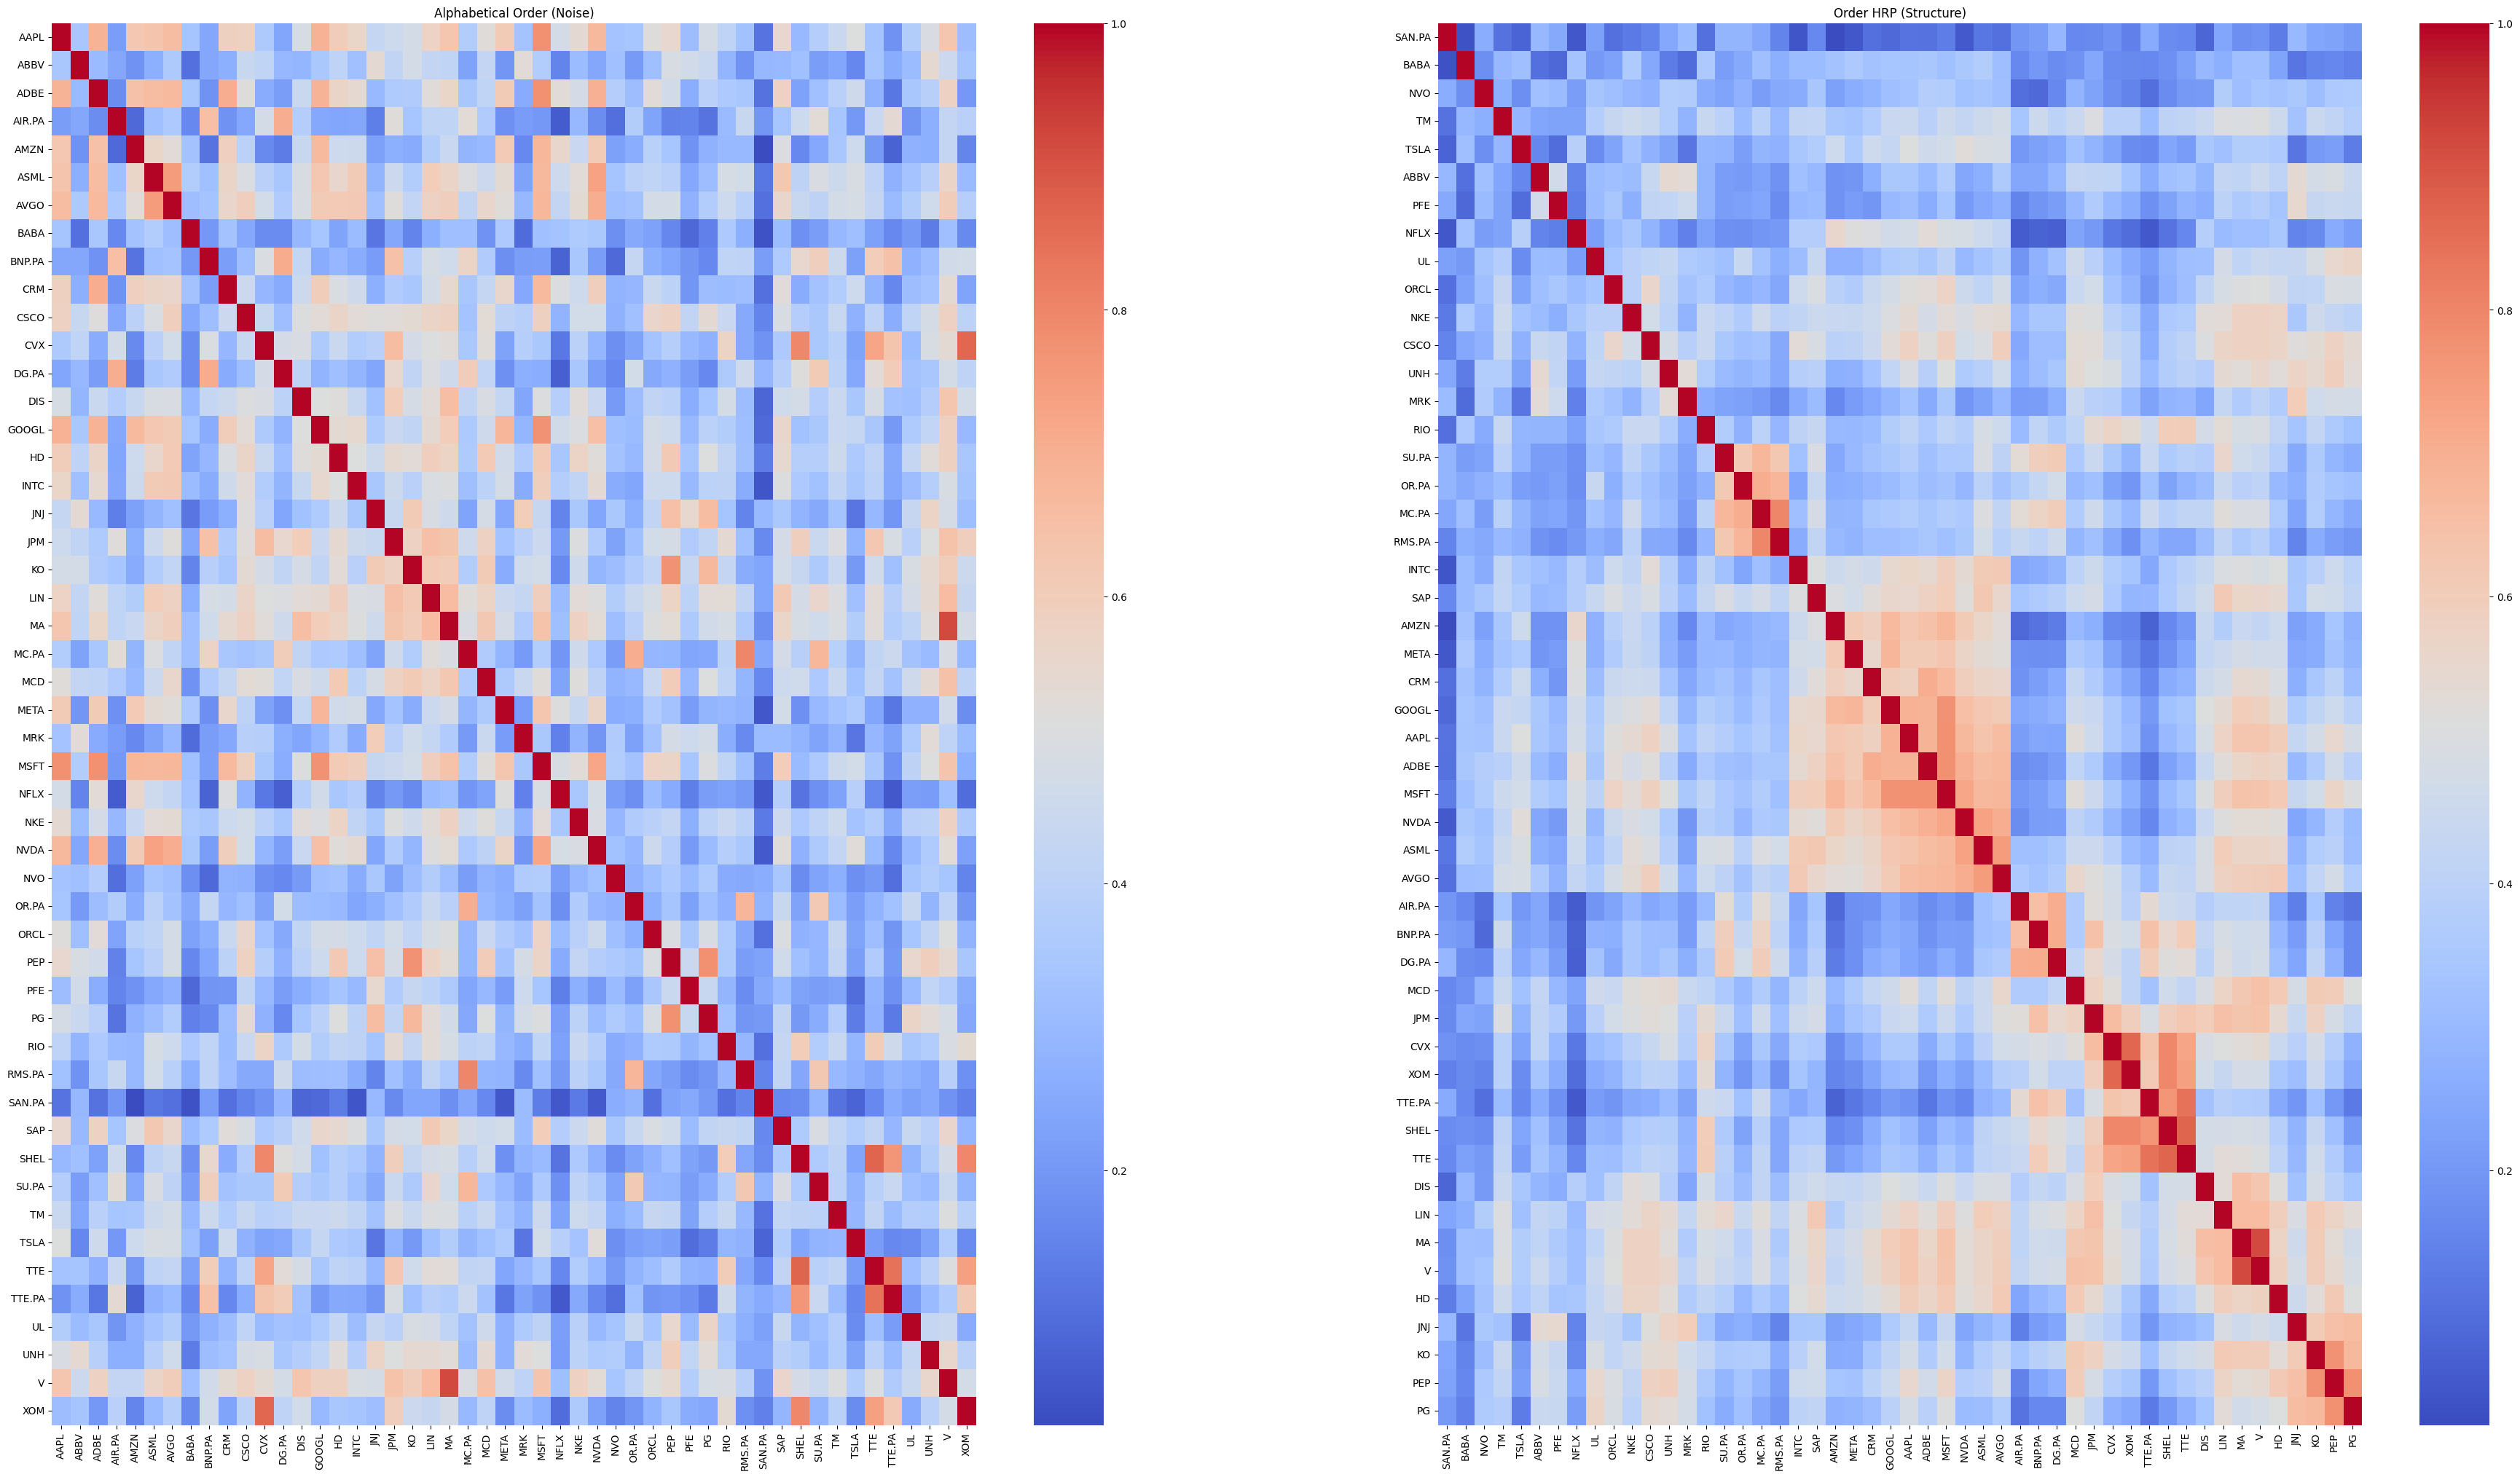
\includegraphics[width=0.5\textwidth]{hrp_heatmap.png}
    \caption{Quasi-diagonalized correlation matrix revealing hierarchical cluster structure}
\end{figure}

\subsection{Empirical Cluster Interpretation}
Figure~5.1 visualizes the quasi-diagonalized correlation matrix for a universe of 50 assets. The hierarchical clustering reveals interpretable sector-based clusters driven by fundamental economic relationships.

The hierarchical clustering identifies a high degree of correlation between \textbf{Procter \& Gamble (PG)}, \textbf{PepsiCo (PEP)},
\textbf{Coca-Cola (KO)}, and \textbf{Johnson \& Johnson (JNJ)}. That is the medium cluster in the low right corner of the heatmap. This cluster represents the \textit{defensive core} of the portfolio, driven by three primary factors:

\begin{itemize} 
    \item \textbf{Sector Homogeneity:} PG, PEP, and KO belong to the Consumer Staples sector, while JNJ exhibits similar non-cyclical behavior within the Healthcare sector. These industries provide essential goods and services with high price inelasticity. 
    \item \textbf{Systemic Risk Sensitivity (Low Beta):} These assets typically exhibit a "risk-off" profile. During periods of market volatility, capital flows into these "safe-haven" stocks due to their predictable cash flows and consistent dividend histories (Dividend Kings). 
    \item \textbf{Common Macroeconomic Drivers:} These firms are globally diversified multinationals sensitive to similar macro variables, such as USD strength and global consumer spending trends, rather than sector-specific technological shifts or cyclical commodity prices. 
\end{itemize}

We can also observe another cluster made up of \textbf{TotalEnergies}, \textbf{Shell}, \textbf{Exxon Mobil} and \textbf{Chevron}. This cluster represents the \textit{energy core} of the portfolio.
\par
Then there is the big cluster made up of \textbf{Broadcom}, \textbf{ASML}, \textbf{NVIDIA}, \textbf{Microsoft}, \textbf{Adobe}, \textbf{Apple}, \textbf{Google}, \textbf{Salesforce}, \textbf{META}, \textbf{Amazon}, \textbf{SAP} and \textbf{Intel}. This cluster represents the \textit{technology core} of the portfolio.
\par

And there is also the cluster made up of \textbf{Hermes}, \textbf{LVMH}, \textbf{L'Oréal} and \textbf{Schneider Electric}.
While \textbf{Schneider Electric (SU.PA)} is fundamentally an industrial leader in energy management and automation, the hierarchical clustering often groups it with luxury giants such as \textbf{LVMH}, \textbf{Hermès}, and \textbf{L'Oréal}. This statistical relationship is driven by the following structural factors:

\begin{itemize} 
    \item \textbf{Index Weighting and "National Champion" Status:} SU.PA is one of the largest constituents of the \textbf{CAC 40}, alongside the luxury stocks. As "national champions" with massive market capitalizations, these stocks are frequently bought and sold together by institutional investors via index-tracking ETFs, leading to high co-movement. 
    \item \textbf{High International Revenue Exposure:} Similar to the luxury sector, over two-thirds of Schneider Electric's revenue is generated outside of France. Both Schneider and the luxury groups are highly sensitive to global trade conditions, the \textbf{USD/EUR exchange rate}, and macroeconomic health in major markets like China and the United States. 
    \item \textbf{Shared Growth Profiles (Premium Valuation):} Schneider Electric often commands a premium valuation multiple (e.g., high P/E ratios) relative to standard industrials due to its exposure to secular growth themes like AI and the energy transition. This causes it to trade more like "growth-oriented" luxury stocks than traditional cyclical capital goods. 
\end{itemize}

\subsection{Recursive Bisection Algorithm}
Once the asset hierarchy is established, HRP constructs portfolio weights through recursive bisection. At each node in the dendrogram, the algorithm splits the asset set into two sub-clusters and allocates capital proportional to the inverse of each cluster's variance.

To do that we consider the covariance matrix of the cluster and get its variance. To get its variance we compute the weights $\mathbf{w}$. 
We get the diagonal elements of the covariance matrix and determine the inverse variance as the vector $\mathbf{v} = \frac{1}{diag}$ and then weights are given by
$\mathbf{w} = \frac{\mathbf{v}}{\mathbf{1}^T \mathbf{v}}$. The variance of the cluster is thus $\mathbf{w}^T \Sigma \mathbf{w}$.

We then compute $\alpha$ such that $\alpha = 1 - \frac{var_{left}}{var_{left} + var_{right}}$.

We then update the weights by multiplying those of the left cluster by $\alpha$ and those of the right cluster by $1 - \alpha$.
Following the principle of a recursive function, this operation is reiterated until the leaf level is reached (cluster size = 1).

\subsection{Properties and Interpretation}
This hierarchical allocation mechanism ensures that highly correlated assets are first grouped as a single risk unit (receiving collective weight allocation), then internally subdivided. Assets with low correlation to all other assets receive higher individual allocations, as they provide unique diversification benefits.

Compared to naive inverse-variance weighting, HRP respects the correlation structure: it penalizes membership in crowded clusters while rewarding isolated positions. The resulting portfolio exhibits lower concentration than equal-weighted or market-cap schemes while maintaining explicit risk balance across the hierarchy.

\section{Comparison}
Lastly let us compared the performance of the three methods and the market weights.
Let us consider the following metrics:
\begin{itemize}
    \item volatility of the portfolio calculated as $\sqrt{\mathbf{w}^T \Sigma \mathbf{w}}$
    \item Herfindahl-Hirschman Index (HHI) of the portfolio calculated as $\sum_{i=1}^N w_i^2$
    \item Diversification Ratio (DR) of the portfolio calculated as $\frac{\sum_{i=1}^N w_i \sqrt{\Sigma_{i,i}}}{\sqrt{\mathbf{w}^T \Sigma \mathbf{w}}}$
\end{itemize}


The views expressed in the Black-Litterman model are the following:
\begin{itemize}
    \item AAPL will have a return of 0.1 with a confidence of 0.3
    \item AAPL and MSFT will overperform GOOGL by 0.02 with a confidence of 0.5
\end{itemize}

The HRP method came first on all metrics. It is the most diversified portfolio, the most stable and has the lowest volatitility.
The Black-Litterman is influenced stongly by views and it comes last with the highest volatility, the lowest risk diverisification and the highest exposure to a single stock.
Finally While the Market-Cap portfolio maintains a lower HHI, indicating a broader spread of capital, the MVO portfolio achieves a superior Diversification Ratio
($DR_{MVO} > DR_{Mkt}$). This suggests that the MVO effectively identified the 'Principal Components' of the covariance matrix to minimize
 the denominator of the DR, whereas the Market-Cap portfolio's concentration in high-beta, highly-correlated mega-cap assets suppressed 
 its diversification benefits.
 It is however important to note her that the HRP method does not try to obtain a specific expected return and focuses only on
 the risk allocation.


\section{Conclusion}

This paper provides a rigorous mathematical foundation for portfolio optimization under estimation risk, 
spanning classical mean-variance theory, Bayesian methods, and graph-theoretic approaches. The unified framework demonstrates how covariance estimation error propagates 
through the optimization problem and motivates three distinct regularization strategies.

The Ledoit-Wolf shrinkage estimator addresses the spectral instability of sample covariance matrices in high-dimensional regimes 
where $N \approx T$. By analytically deriving the optimal shrinkage intensity $\delta^* = (\pi - \rho)/\gamma$, we stabilize the KKT system 
and prevent corner solutions driven by eigenvalue estimation noise. The finite-sample correction $\hat{\delta}^* \sim O(1/T)$ ensures asymptotic consistency 
while providing maximum stabilization when data is scarce.

The Black-Litterman model offers a Bayesian alternative, allowing practitioners to blend market equilibrium priors with subjective views through precision-weighted updates. 
The scaling factor $\tau \in [0.01, 0.05]$ reflects the statistical principle that mean estimates exhibit lower variance than individual observations, preventing over-reaction to speculative forecasts. 
Our empirical comparison reveals that aggressive view incorporation (low confidence thresholds) can dominate diversification benefits, leading to concentrated portfolios with elevated volatility.

Hierarchical Risk Parity circumvents the expected return estimation problem entirely by imposing risk parity through recursive bisectioning along the asset correlation hierarchy. 
The correlation distance metric $d_{i,j} = \sqrt{0.5(1-\rho_{i,j})}$ satisfies the triangle inequality and maps naturally to Euclidean geometry in standardized return space. 
HRP emerged as the most robust method in our empirical tournament, achieving superior diversification metrics (lowest HHI, highest Diversification Ratio) and minimal sensitivity to estimation windows.

The comparison section underscores a fundamental tension in quantitative portfolio construction: mean-variance optimization seeks to maximize risk-adjusted returns but remains vulnerable to estimation error; 
HRP sacrifices return targeting for stability. The choice between methods depends critically on the investor's confidence in return forecasts, the quality of available data ($T$ relative to $N$), 
and tolerance for rebalancing costs induced by parameter instability.

Future work should extend this framework to incorporate transaction costs, dynamic rebalancing strategies, and regime-switching covariance models. 
The interplay between shrinkage intensity and portfolio turnover warrants further investigation, as does the integration of machine learning-based covariance estimators with classical portfolio theory.

The mathematical derivations and empirical validations presented here provide practitioners with a comprehensive toolkit for constructing robust portfolios in the face of pervasive estimation uncertainty.

\end{document}
